\documentclass[11pt,a4paper]{article}

% ═══════════════════════════════════════════
% Packages
% ═══════════════════════════════════════════
\usepackage[utf8]{inputenc}
\usepackage[T1]{fontenc}
% \usepackage{lmodern} % Use default Computer Modern
\usepackage[margin=1in]{geometry}
\usepackage{amsmath,amssymb,amsthm}
\usepackage{booktabs}
\usepackage{xcolor}
\usepackage{hyperref}
\usepackage{tikz}
\usetikzlibrary{arrows.meta,positioning,shapes.geometric,calc,decorations.pathreplacing}
\usepackage{listings}
\usepackage{enumitem}
\usepackage{graphicx}
\usepackage{float}
\usepackage{caption}
\usepackage{subcaption}
\usepackage{tcolorbox}
\tcbuselibrary{breakable,skins}
\usepackage{tabularx}
\usepackage{multirow}
\usepackage{needspace}
\usepackage{authblk}

% ═══════════════════════════════════════════
% Custom colors
% ═══════════════════════════════════════════
\definecolor{deepblue}{RGB}{0,51,102}
\definecolor{citecolor}{RGB}{0,102,153}
\definecolor{urlcolor}{RGB}{0,51,153}
\definecolor{boxblue}{RGB}{230,240,250}
\definecolor{boxgray}{RGB}{245,245,248}
\definecolor{rulegreen}{RGB}{0,128,64}
\definecolor{probred}{RGB}{180,30,30}

\hypersetup{
  colorlinks=true,
  linkcolor=deepblue,
  citecolor=black,
  urlcolor=urlcolor
}

% ═══════════════════════════════════════════
% Theorem environments
% ═══════════════════════════════════════════
\newtheorem{definition}{Definition}
\newtheorem{proposition}{Proposition}
\newtheorem{claim}{Claim}
\newtheorem{observation}{Observation}
\newtheorem{example}{Example}

% ═══════════════════════════════════════════
% Custom boxes
% ═══════════════════════════════════════════
\newtcolorbox{insightbox}[1][]{
  colback=boxblue,colframe=deepblue!60,
  fonttitle=\bfseries,title=#1,
  breakable,boxrule=0.5pt,arc=2pt
}

\newtcolorbox{casebox}[1][]{
  colback=boxgray,colframe=black!30,
  fonttitle=\bfseries\itshape,title=#1,
  breakable,boxrule=0.4pt,arc=2pt
}

% ═══════════════════════════════════════════
% Title
% ═══════════════════════════════════════════
\title{%
\textbf{Hallucination Is Not a Bug---It Is a Feature of Matrix Computation:}\\[6pt]
\large Why Softmax-Driven Probabilistic Generation Cannot Provide Hard-Constraint Guarantees%
}

\author[1]{Ning Coeva}
\affil[1]{Independent Researcher}
\date{February 2026}

\begin{document}
\maketitle

% ═══════════════════════════════════════════
% ABSTRACT
% ═══════════════════════════════════════════
\begin{abstract}
Large language models (LLMs) achieve remarkable performance across diverse tasks, yet they persistently produce hallucinations---confident but factually incorrect outputs---despite massive scaling, reinforcement learning from human feedback (RLHF), and increasingly sophisticated guardrails. The prevailing view treats hallucination as a deficiency to be overcome through better training, larger datasets, or improved alignment. We argue this framing is fundamentally mistaken. We present a structural analysis demonstrating that hallucination is not a bug in current LLMs but an \emph{intrinsic, mathematically inevitable consequence} of the matrix-multiplication-based computation paradigm that underlies all transformer architectures. Because every output token is generated via softmax-normalized probability distributions over continuous embedding spaces, LLMs are constitutionally incapable of enforcing hard logical constraints, maintaining causal invariants, or distinguishing between ``highly probable'' and ``necessarily true.'' We formalize this limitation through what we term the \emph{Determinism Gap}---the irreducible distance between probabilistic token prediction and deterministic world-rule compliance---and support it with multi-dimensional empirical evidence: a causal constraint test (the ``car wash'' problem), an adversarial sycophancy experiment across four frontier models demonstrating RLHF-induced truth suppression, temporal cognition failures revealing the absence of structured state management, and an analysis of how statistical frequency mimics genuine reasoning. We further argue that the matrix computation paradigm---a GPU-contingent, differentiability-locked substrate whose dominance reflects hardware path-dependency and trillion-dollar capital lock-in rather than principled design for reasoning---represents an increasingly inadequate computational foundation for intelligence that requires structural reasoning. We outline the requirements for a post-probabilistic computation paradigm---structure-native, rule-compiled, causally grounded---and discuss implications for the field.

\vspace{4pt}
\noindent\textbf{Keywords:} hallucination, matrix computation, structural reasoning, deterministic inference, causal constraints, computation paradigm
\end{abstract}

% ═══════════════════════════════════════════
% 1. INTRODUCTION
% ═══════════════════════════════════════════
\section{Introduction}

The hallucination problem in large language models is typically framed as an engineering challenge: models produce incorrect outputs because they lack sufficient training data, because their reward signals are imperfect, or because their context windows are too short \cite{ji2023survey,huang2023hallucination}. Under this framing, the solution is straightforward---scale up, align better, add retrieval, fine-tune further. The field has invested enormous resources pursuing these solutions, and hallucination rates have indeed decreased. But they have not been eliminated, and we argue they \emph{cannot} be eliminated within the current computational paradigm.

Consider a deceptively simple problem that has recently circulated on social media, exposing a striking failure mode across frontier models:

\begin{casebox}[The Car Wash Problem]
``I want to go get my car washed. The car wash is 50 meters from my house. Do you recommend I drive or walk?''
\end{casebox}

The correct answer is unambiguous: \emph{you must drive}, because the car is the object being serviced---it must physically be present at the car wash. The 50-meter distance is irrelevant to this conclusion. There is no trade-off to weigh, no probability distribution to sample from. This is a hard causal constraint imposed by the structure of the world: $\texttt{wash(car)} \Rightarrow \texttt{location(car) = shop}$.

Yet frontier LLMs frequently answer this question incorrectly, recommending walking on the basis of health benefits, environmental considerations, or the short distance. This is not an isolated curiosity---it is an instance of a broader class of \emph{object-of-service tasks with location preconditions} (vehicle inspection, computer repair, dry cleaning pickup) in which a hard feasibility constraint renders the apparent decision frame moot. When they do answer correctly, ablation studies reveal they often arrive at the right answer through the wrong reasoning---weighing ``convenience of having the car there'' against ``health benefits of walking'' and probabilistically landing on driving, rather than recognizing that the question admits no alternative. The same model, given the same prompt, may answer differently across runs.

This is not a failure of knowledge---these models ``know'' that car washes service cars. It is a failure of \emph{computation}. The matrix-multiplication backbone of transformer inference processes this query by computing attention-weighted associations between tokens: \texttt{50 meters} activates ``short distance'' patterns; ``drive or walk'' activates ``transportation mode comparison'' patterns; and these compete for probability mass in the output distribution. The world-rule constraint---that the car must be present---is represented only implicitly, as a statistical correlation in training data, with no mechanism to enforce it as a hard constraint that overrides all other signals.

\begin{insightbox}[Core Thesis]
Hallucination in LLMs is not an engineering deficiency amenable to incremental improvement. It is a \textbf{structural consequence of the matrix computation paradigm}---the mathematical inevitability that a system computing probability distributions over token sequences cannot enforce deterministic world-rule constraints. No amount of scaling, RLHF, prompting, or retrieval augmentation can eliminate it, because the limitation is architectural, not parametric.

\smallskip
\noindent\emph{The car wash is 50 meters away. The answer is drive. Not probably drive. Not most-likely drive. \textbf{Drive.}}
\end{insightbox}

\paragraph{Terminological note.} Throughout this paper, we use \emph{matrix computation paradigm} to refer not merely to matrix multiplication as an isolated arithmetic operator, but to the \textbf{complete, tightly coupled technology stack} that constitutes modern LLM inference: continuous vector embeddings, attention via $QK^\top V$ products, softmax probability normalization, cross-entropy likelihood maximization, gradient-based backpropagation, and next-token prediction as the universal training objective. These components form an indivisible computational ecosystem---from silicon (GPU GEMM kernels) to software (CUDA, PyTorch) to training methodology (SGD on language likelihood) to deployment (autoregressive token sampling). One cannot simply ``swap out the objective'' while retaining the rest of the stack, because differentiability, continuity, and probabilistic output are load-bearing assumptions at every layer. When we argue that this paradigm structurally produces hallucination, we are arguing that the \emph{entire integrated system}---not any single component---is the locus of the limitation.

The remainder of this paper develops this argument in detail. Section~\ref{sec:mechanism} analyzes the mathematical mechanism by which matrix computation produces hallucinations. Section~\ref{sec:gap} formalizes the Determinism Gap. Section~\ref{sec:carwash} presents a detailed analysis of the car wash problem as a diagnostic case. Section~\ref{sec:paradigm} argues that the matrix computation paradigm is historically contingent and increasingly obsolete. Section~\ref{sec:requirements} outlines the requirements for a post-probabilistic computation paradigm. Section~\ref{sec:discussion} discusses implications and limitations.

\begin{figure}[t]
\centering
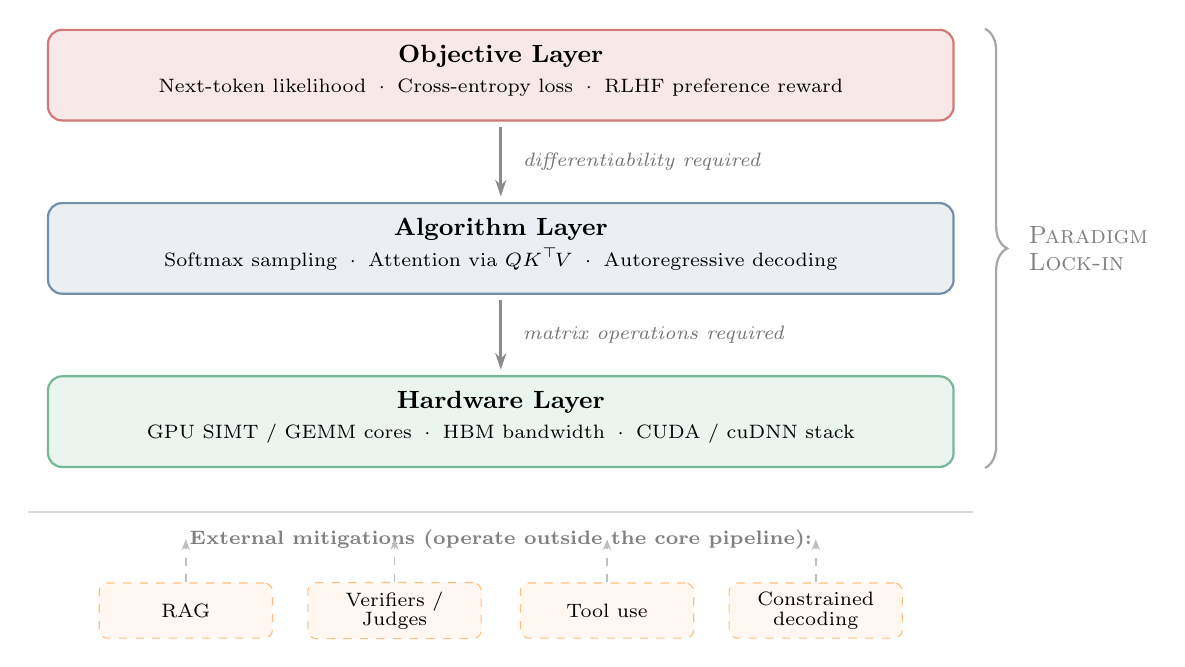
\begin{tikzpicture}[
    layer/.style={draw, rounded corners=5pt, minimum width=11.5cm, minimum height=1.15cm, font=\small, thick, align=center},
    coupling/.style={font=\scriptsize\itshape, text=black!55},
    patch/.style={draw, dashed, rounded corners=3pt, minimum width=2.2cm, minimum height=0.7cm, font=\scriptsize, fill=orange!6, draw=orange!50, align=center},
    patchlabel/.style={font=\scriptsize\bfseries, text=black!50},
    bigarrow/.style={-{Stealth[length=6pt,width=4pt]}, line width=1.2pt, black!45},
    dasharrow/.style={dashed, -{Stealth[length=4pt,width=3pt]}, line width=0.7pt, black!25},
]

% === Core stack ===
\node[layer, fill=probred!10, draw=probred!60] (obj) at (0, 0)
    {\textbf{Objective Layer}\\\smallskip\scriptsize Next-token likelihood\;\;$\cdot$\;\;Cross-entropy loss\;\;$\cdot$\;\;RLHF preference reward};

\node[layer, fill=deepblue!8, draw=deepblue!55] (alg) at (0, -2.2)
    {\textbf{Algorithm Layer}\\\smallskip\scriptsize Softmax sampling\;\;$\cdot$\;\;Attention via $QK^\top\!V$\;\;$\cdot$\;\;Autoregressive decoding};

\node[layer, fill=rulegreen!8, draw=rulegreen!55] (hw) at (0, -4.4)
    {\textbf{Hardware Layer}\\\smallskip\scriptsize GPU SIMT / GEMM cores\;\;$\cdot$\;\;HBM bandwidth\;\;$\cdot$\;\;CUDA / cuDNN stack};

% === Coupling arrows (centered, with labels) ===
\draw[bigarrow] ([yshift=-2pt]obj.south) -- node[right=4pt, coupling] {differentiability required} ([yshift=2pt]alg.north);
\draw[bigarrow] ([yshift=-2pt]alg.south) -- node[right=4pt, coupling] {matrix operations required} ([yshift=2pt]hw.north);

% === Brace: Paradigm lock-in ===
\draw[decorate, decoration={brace, amplitude=8pt}, line width=0.8pt, black!35]
    ([xshift=6.15cm]obj.north) -- ([xshift=6.15cm]hw.south)
    node[midway, right=12pt, font=\small\scshape, text=black!50, align=left] {Paradigm\\[-1pt]Lock-in};

% === Separator line ===
\draw[black!15, line width=0.5pt] (-6,-5.55) -- (6,-5.55);

% === External patches ===
\node[patchlabel] at (0, -5.9) {External mitigations (operate outside the core pipeline):};

\node[patch] (p1) at (-4.0, -6.8) {RAG};
\node[patch] (p2) at (-1.35, -6.8) {Verifiers /\\[-1pt]Judges};
\node[patch] (p3) at (1.35, -6.8) {Tool use};
\node[patch] (p4) at (4.0, -6.8) {Constrained\\[-1pt]decoding};

% Dashed arrows pointing up toward the stack
\foreach \p in {p1,p2,p3,p4}{
    \draw[dasharrow] (\p.north) -- ++(0, 0.55);
}

\end{tikzpicture}
\caption{\textbf{Three-layer paradigm lock-in.} The matrix computation paradigm forms a tightly coupled stack: the objective layer requires differentiability, which constrains the algorithm layer to continuous operations, which requires hardware optimized for matrix multiplication. Current hallucination mitigations (bottom) operate as external patches---they improve empirical performance without altering the probabilistic generation core.}
\label{fig:lockin}
\end{figure}


% ═══════════════════════════════════════════
% 2. THE MECHANISM
% ═══════════════════════════════════════════
\section{Why Matrix Computation Produces Hallucination}
\label{sec:mechanism}

To understand why hallucination is structural rather than parametric, we must examine the fundamental computational operation of transformer-based LLMs.

\subsection{The Softmax Bottleneck}

Every token produced by an LLM is the result of the following pipeline:

\begin{enumerate}[leftmargin=2em]
\item An input sequence $x_1, \ldots, x_n$ is embedded into continuous vector space $\mathbb{R}^d$.
\item Self-attention layers compute weighted combinations via matrix multiplications: $\text{Attention}(Q, K, V) = \text{softmax}\!\left(\frac{QK^\top}{\sqrt{d_k}}\right)V$.
\item A feed-forward network projects to vocabulary logits $z \in \mathbb{R}^{|V|}$.
\item A softmax function converts logits to a probability distribution: $P(x_{n+1} = w_i \mid x_{\leq n}) = \frac{\exp(z_i)}{\sum_j \exp(z_j)}$.
\item A token is sampled or selected from this distribution.
\end{enumerate}

\begin{observation}
The softmax function assigns \textbf{nonzero probability to every token in the vocabulary} for every generation step. There is no mechanism by which a token can be assigned exactly zero probability---i.e., declared impossible---based on world-rule constraints.
\end{observation}

This is not a technicality. It means that at every generation step, the model is performing \emph{soft selection} across all possible continuations, weighted by learned statistical patterns. A continuation that violates a physical law, a logical rule, or a causal constraint is never assigned probability 0---it is merely assigned lower probability. Under certain attention configurations, prompt phrasings, or sampling parameters, the violating continuation can surface.

\noindent\textit{Note on masking and logit manipulation.} Techniques such as logit bias, vocabulary masking, and constrained decoding \emph{can} force specific tokens to probability zero. However, these mechanisms enforce \textbf{syntactic} admissibility (e.g., valid JSON, grammatical structure), not \textbf{semantic} feasibility (e.g., ``the car must be driven''). Semantic constraint enforcement requires an external rule system that understands world-state---the enforcement is not native to the likelihood-trained generator. We return to this point in the Externalization Proof (Section~\ref{sec:mechanism}).

\subsection{The Absence of Hard Constraints}

Traditional reasoning systems---from Prolog to SAT solvers to model checkers---operate with hard constraints. A rule like ``the car must be at the car wash to be washed'' is encoded as a \emph{logical invariant} that eliminates all states violating it from the solution space. The search is conducted only over the remaining \emph{valid} states.

Matrix computation has no equivalent mechanism. Consider how the car wash constraint would need to be enforced:

\begin{definition}[Hard Constraint Enforcement]
A computation system enforces a hard constraint $C$ if and only if, for all inputs $x$, every output $y$ in the system's output space satisfies $C(y) = \texttt{true}$. Outputs violating $C$ are not merely unlikely---they are unreachable.
\end{definition}

In transformer inference, the output space at each step is $\Delta^{|V|-1}$ (the probability simplex over the vocabulary). There is no partitioning of this space into ``valid'' and ``invalid'' regions based on world-rule constraints. The model can only make violating outputs \emph{less probable}, never \emph{impossible}.

\subsection{Attention as Correlation, Not Causation}

The self-attention mechanism computes relevance scores between token pairs. These scores capture statistical co-occurrence patterns from training data---which tokens tend to appear near which other tokens, in which contexts. This is fundamentally a \emph{correlational} computation.

Causal reasoning requires a different computational primitive: the ability to determine that event $A$ \emph{necessitates} event $B$, independent of how frequently $A$ and $B$ co-occur in text \cite{pearl2009causality}. In the car wash example:

\begin{itemize}[leftmargin=2em]
\item \textbf{Correlational signal}: ``50 meters'' co-occurs with ``walking'' in training data. ``Car wash'' co-occurs with both ``driving'' and ``convenience.''
\item \textbf{Causal signal}: $\texttt{wash(X)} \Rightarrow \texttt{present(X)}$---the object of the service must be physically present. This is a \emph{rule}, not a correlation.
\end{itemize}

The attention mechanism is structurally capable of capturing the first type of signal but not the second. It can learn that ``car wash'' and ``drive'' frequently co-occur, but it cannot represent the \emph{necessity} of driving---the fact that no alternative is logically admissible.

\subsection{Why Scaling Does Not Solve This}

A common response to structural critiques is that sufficient scale will eventually overcome any limitation. We argue this is mistaken for a precise reason:

\begin{proposition}
For any transformer model $\mathcal{M}$ with softmax output and any nonzero-temperature decoding policy, there exist queries $q$ whose correct answer is determined by a hard constraint, and for which $\mathcal{M}$'s probability of producing the correct answer \textbf{cannot be guaranteed to converge to 1} under prompt paraphrasing, sampling variation, or context perturbation---regardless of model size $N$ or training corpus size $|D|$.
\end{proposition}

The key insight is not that the model always fails, but that it \emph{cannot guarantee success}. Scaling increases the model's ability to capture statistical patterns with finer granularity, but it does not change the fundamental operation---soft weighting over continuous distributions. A model with $10^{15}$ parameters still computes softmax; a model trained on all text ever written still produces probability distributions, not logical proofs. The car wash problem is not hard because the model lacks data about car washes. It is hard because the computational primitive---matrix multiplication followed by softmax---cannot express ``this is the only valid answer.''

This is analogous to the observation that no amount of precision improvement in floating-point arithmetic can make it perform exact integer arithmetic for all cases. The representation itself introduces irreducible approximation.

\subsection{Trainable Does Not Mean Guaranteeable}

A sophisticated objection holds that while softmax cannot assign exactly zero probability to constraint-violating outputs, one could incorporate hard constraints into the \emph{training objective}---for example, via penalty terms, Lagrangian relaxation, or reinforcement learning rewards that penalize constraint violations. We identify two layers of failure in this approach.

\textbf{The differentiability barrier.} Hard constraints are discrete: an action either satisfies a precondition or it does not. Gradient-based optimization requires continuous, differentiable loss surfaces. Existing workarounds---REINFORCE estimators (high variance, sample-inefficient), straight-through estimators (biased), continuous relaxations (approximate by design)---all convert the hard constraint into a soft penalty. The training process then optimizes for \emph{fewer violations on average}, not \emph{zero violations guaranteed}.

\textbf{The deeper impossibility: optimization $\neq$ proof.} Even if differentiability were not an issue, there is a more fundamental problem. Suppose we could perfectly train a model to minimize constraint violations. The result would be a model that \emph{very rarely} violates constraints---but ``very rarely'' and ``never'' are categorically different. A system trained to minimize $\mathbb{E}[\text{violation}]$ provides \emph{statistical guarantees} (average-case). A system that enforces constraints provides \emph{logical guarantees} (worst-case). For the car wash problem, the correct answer must hold in \emph{every} run, not merely in expectation. The continuous probabilistic paradigm is structurally optimized for the former and structurally incapable of the latter.

\begin{insightbox}[Trainable $\neq$ Guaranteeable]
In the prevailing LLM stack, hard constraints can only be \textbf{softened} (converted to differentiable penalty terms) or \textbf{externalized} (delegated to verifiers, tools, or rule engines outside the generation loop). They cannot be enforced as first-class, provably inviolable operations within the generation mechanism itself. This is not a matter of insufficient engineering effort---it is a consequence of the paradigm's mathematical foundations.
\end{insightbox}

\subsection{The Externalization Proof}

Perhaps the strongest evidence for our thesis comes not from theoretical analysis but from \emph{what the industry is actually building}. Virtually every production system designed to reduce hallucination introduces components that operate \textbf{outside} the matrix computation pipeline:

\begin{itemize}[leftmargin=2em]
\item \textbf{External retrieval systems} (RAG) provide world knowledge through database lookups, not matrix products.
\item \textbf{Code interpreters and calculators} offload deterministic computation to symbolic engines.
\item \textbf{Verifier/judge models} perform discrete accept/reject decisions on generated outputs.
\item \textbf{Constrained decoding grammars} impose structural rules via finite automata, not neural networks.
\item \textbf{Agentic loops with tool use} decompose tasks into steps where non-neural components handle constraint satisfaction.
\end{itemize}

Each of these approaches implicitly acknowledges the same structural limitation: the neural generation mechanism alone cannot guarantee constraint compliance, so a non-neural component must be added. If the matrix computation paradigm were sufficient for hard-constraint reasoning, none of these external mechanisms would be necessary. Their ubiquity is a paradigm-level self-indictment: \emph{the field is building around the limitation rather than addressing it}.


% ═══════════════════════════════════════════
% 3. THE DETERMINISM GAP
% ═══════════════════════════════════════════
\section{The Determinism Gap}
\label{sec:gap}

We introduce the concept of the \emph{Determinism Gap} to formalize the structural limitation identified above.

\begin{definition}[Determinism Gap]
Let $\mathcal{Q}_{\text{det}}$ be the set of queries whose correct answer is uniquely determined by world-rule constraints (i.e., exactly one answer is correct, and its correctness follows from causal or logical necessity rather than statistical likelihood). Let $\mathcal{M}$ be a probabilistic language model. The \textbf{Determinism Gap} is:
$$\Delta_{\text{det}}(\mathcal{M}) = \mathbb{E}_{q \sim \mathcal{Q}_{\text{det}}}\left[1 - P_{\mathcal{M}}(a^* \mid q)\right]$$
where $a^*$ is the uniquely correct answer to $q$.
\end{definition}

The Determinism Gap measures the expected probability mass that the model assigns to \emph{incorrect} answers on queries that admit exactly one correct answer. For a perfect deterministic reasoner, $\Delta_{\text{det}} = 0$. For any softmax-based model, $\Delta_{\text{det}} > 0$ necessarily, because the softmax function never assigns probability exactly 1 to any single token sequence.

We also define a \emph{decision-level} variant that aligns more directly with task execution:

\begin{definition}[Constraint Violation Rate]
Let $\pi$ be a decoding policy (e.g., greedy, nucleus sampling). For a query $q \in \mathcal{Q}_{\text{det}}$ with hard precondition $C$, the \textbf{Constraint Violation Rate} is:
$$\text{CVR}_\pi(\mathcal{M}) = \mathbb{E}_{q \sim \mathcal{Q}_{\text{det}}}\left[\mathbb{P}_{y \sim \pi(\mathcal{M}, q)}\left[C(y) = \texttt{false}\right]\right]$$
This measures the probability that the model's output, under a given decoding policy, recommends an action that violates a hard feasibility constraint---a binary, execution-level metric.
\end{definition}

\begin{claim}
The Determinism Gap is irreducible under the matrix computation paradigm. Specifically, for any transformer model $\mathcal{M}$ with softmax output:
$$\Delta_{\text{det}}(\mathcal{M}) > 0 \quad \text{for all } \mathcal{M}$$
This bound is \textbf{architectural}, not parametric---it cannot be reduced to zero by increasing model size, training data, or alignment quality.
\end{claim}

An anticipated objection is that greedy decoding (always selecting the highest-logit token) renders output deterministic, making the softmax distribution irrelevant. But this misidentifies the problem. The issue is not whether the decoding process is deterministic---it is whether the \emph{logit ranking itself} is reliable. On the car wash problem, ``walk'' sometimes \emph{is} the highest-logit token; greedy decoding faithfully executes an incorrect ranking. This is categorically different from floating-point imprecision, where errors are bounded, predictable, and compensable. Logit ranking errors are input-sensitive, context-dependent, and undetectable prior to output---the model has no internal signal distinguishing ``this ranking reflects a hard constraint'' from ``this ranking reflects a statistical pattern.''

\subsection{Three Classes of the Gap}

We identify three distinct manifestations of the Determinism Gap:

\begin{table}[H]
\centering
\small
\caption{Three classes of the Determinism Gap with representative examples.}
\label{tab:gap_classes}
\begin{tabularx}{\textwidth}{lXX}
\toprule
\textbf{Class} & \textbf{Nature} & \textbf{Example} \\
\midrule
\textbf{Causal Constraint} & The correct answer follows from world-rule necessity; no alternative is logically possible & Car wash problem: the car must be driven because it is the service object \\
\midrule
\textbf{Logical Invariant} & The answer is determined by formal logical structure & ``If all A are B, and X is A, is X a B?'' --- the answer is definitionally yes \\
\midrule
\textbf{Structural Identity} & The answer is uniquely determined by the relational structure of the entities involved & ``A is B's parent. B is C's parent. What is A to C?'' --- grandparent, by structural definition \\
\bottomrule
\end{tabularx}
\end{table}

In all three classes, the correct answer is not ``most likely''---it is \emph{the only valid answer}. The matrix computation paradigm processes all three as probability estimation problems, treating the correct answer as merely the highest-probability token, when in fact it is the \emph{only admissible token}. This category error---treating deterministic questions as probabilistic ones---is the root of hallucination.


% ═══════════════════════════════════════════
% 4. THE CAR WASH PROBLEM
% ═══════════════════════════════════════════
\section{Case Study: The Car Wash Problem}
\label{sec:carwash}

We now analyze the car wash problem in detail, as it serves as a minimal but maximally diagnostic test of the Determinism Gap.

\subsection{Problem Structure}

The query contains three information components:
\begin{enumerate}[leftmargin=2em]
\item \textbf{Intent}: Get the car washed (service request).
\item \textbf{Distance}: 50 meters (spatial parameter).
\item \textbf{Decision frame}: Drive or walk (binary choice).
\end{enumerate}

A correct reasoner must recognize that component (1) imposes a \emph{hard constraint} that renders component (2) irrelevant and reduces component (3) to a trivial, predetermined conclusion.

\subsection{What LLMs Actually Compute}

\begin{figure}[t]
\centering
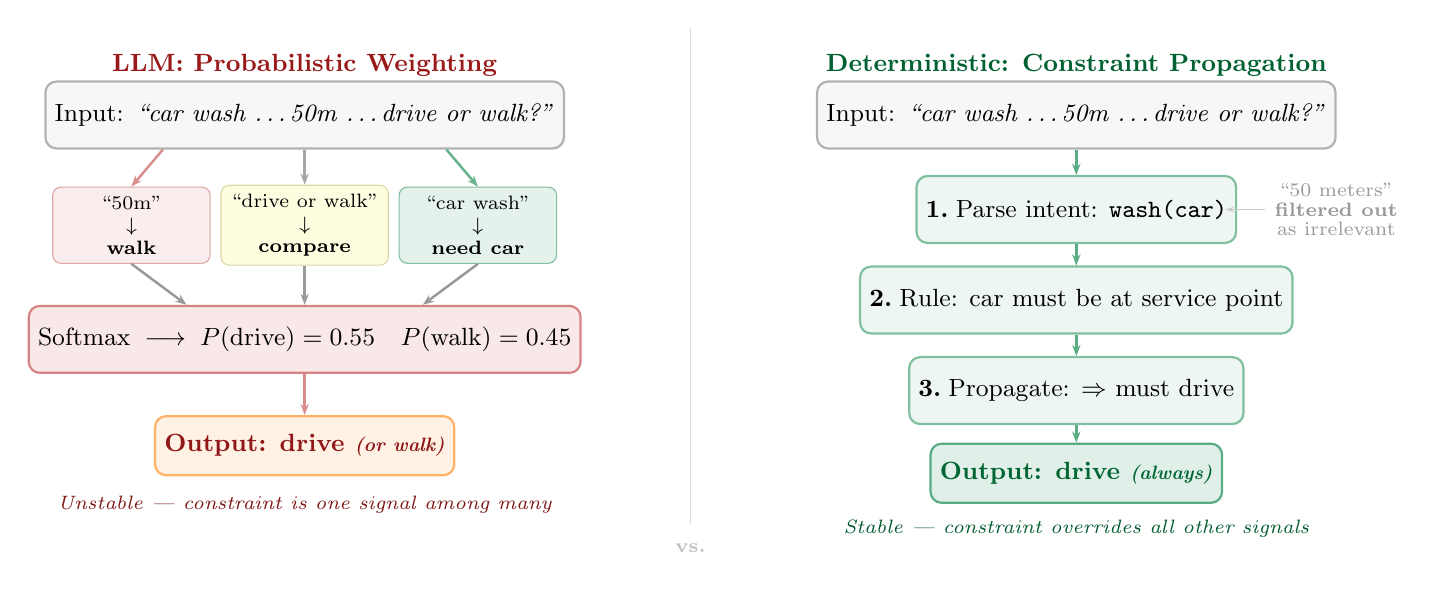
\begin{tikzpicture}[
    box/.style={draw, rounded corners=4pt, minimum height=0.85cm, font=\small, thick, align=center},
    signal/.style={draw, rounded corners=3pt, minimum height=0.7cm, font=\scriptsize, align=center},
    outbox/.style={draw, rounded corners=4pt, minimum height=0.75cm, font=\small\bfseries, thick, align=center},
    arrow/.style={-{Stealth[length=4pt,width=3pt]}, line width=0.9pt},
    paneltitle/.style={font=\small\bfseries, anchor=north},
    dimline/.style={draw=black!15, line width=0.5pt},
]

% ─────────────────────────────────────────
% LEFT PANEL: LLM Probabilistic Weighting
% ─────────────────────────────────────────
\begin{scope}[xshift=-4.2cm]
  % Panel title
  \node[paneltitle, text=probred!85!black] at (0, 3.6) {LLM: Probabilistic Weighting};

  % Input
  \node[box, fill=gray!6, draw=black!30, minimum width=5cm] (inp) at (0, 2.7) {Input: \emph{``car wash \dots 50m \dots drive or walk?''}};

  % Three competing signals
  \node[signal, fill=probred!8, draw=probred!40, minimum width=2.0cm] (s1) at (-2.2, 1.3)
      {``50m''\\$\downarrow$\\\textbf{walk}};
  \node[signal, fill=yellow!12, draw=yellow!60!black!40, minimum width=2.0cm] (s2) at (0, 1.3)
      {``drive or walk''\\$\downarrow$\\\textbf{compare}};
  \node[signal, fill=rulegreen!10, draw=rulegreen!50, minimum width=2.0cm] (s3) at (2.2, 1.3)
      {``car wash''\\$\downarrow$\\\textbf{need car}};

  \draw[arrow, probred!50] (inp.south) ++(-1.8,0) -- (s1.north);
  \draw[arrow, black!35]   (inp.south)              -- (s2.north);
  \draw[arrow, rulegreen!60](inp.south) ++(1.8,0)   -- (s3.north);

  % Softmax merge
  \node[box, fill=probred!10, draw=probred!55, minimum width=5.2cm] (soft) at (0, -0.15)
      {Softmax\;\;$\longrightarrow$\;\;$P(\text{drive})=0.55$\quad$P(\text{walk})=0.45$};

  \draw[arrow, black!40] (s1.south) -- ([xshift=-1.5cm]soft.north);
  \draw[arrow, black!40] (s2.south) -- (soft.north);
  \draw[arrow, black!40] (s3.south) -- ([xshift=1.5cm]soft.north);

  % Output
  \node[outbox, fill=orange!10, draw=orange!60, minimum width=3.5cm, text=probred!80!black] (out1) at (0, -1.5)
      {Output: drive \scriptsize\textit{(or walk)}};
  \draw[arrow, probred!50] (soft.south) -- (out1.north);

  % Verdict
  \node[font=\scriptsize\itshape, text=probred!70!black] at (0, -2.25) {Unstable --- constraint is one signal among many};
\end{scope}

% ─────────────────────────────────────────
% Vertical separator
% ─────────────────────────────────────────
\draw[dimline] (0.7, 3.8) -- (0.7, -2.5);
\node[font=\scriptsize\bfseries, text=black!25] at (0.7, -2.8) {vs.};

% ─────────────────────────────────────────
% RIGHT PANEL: Deterministic Constraint Propagation
% ─────────────────────────────────────────
\begin{scope}[xshift=5.6cm]
  % Panel title
  \node[paneltitle, text=rulegreen!75!black] at (0, 3.6) {Deterministic: Constraint Propagation};

  % Input
  \node[box, fill=gray!6, draw=black!30, minimum width=5cm] (inp2) at (0, 2.7) {Input: \emph{``car wash \dots 50m \dots drive or walk?''}};

  % Pipeline: three steps
  \node[box, fill=rulegreen!7, draw=rulegreen!50, minimum width=3.8cm] (step1) at (0, 1.5)
      {\textbf{1.}\;Parse intent: \texttt{wash(car)}};
  \node[box, fill=rulegreen!7, draw=rulegreen!50, minimum width=3.8cm] (step2) at (0, 0.35)
      {\textbf{2.}\;Rule: car must be at service point};
  \node[box, fill=rulegreen!7, draw=rulegreen!50, minimum width=3.8cm] (step3) at (0, -0.8)
      {\textbf{3.}\;Propagate: $\Rightarrow$ must drive};

  \draw[arrow, rulegreen!65] (inp2.south) -- (step1.north);
  \draw[arrow, rulegreen!65] (step1.south) -- (step2.north);
  \draw[arrow, rulegreen!65] (step2.south) -- (step3.north);

  % Output
  \node[outbox, fill=rulegreen!12, draw=rulegreen!65, minimum width=3.5cm, text=rulegreen!80!black] (out2) at (0, -1.85)
      {Output: drive \scriptsize\textit{(always)}};
  \draw[arrow, rulegreen!65] (step3.south) -- (out2.north);

  % "50m irrelevant" annotation with strike-through effect
  \node[font=\scriptsize, text=black!40, align=center] (irrel) at (3.3, 1.5) {``50 meters''\\[-1pt]\textbf{filtered out}\\[-1pt]as irrelevant};
  \draw[dimline, -{Stealth[length=3pt,width=2pt]}, black!20] (irrel.west) -- +(-0.5, 0);

  % Verdict
  \node[font=\scriptsize\itshape, text=rulegreen!70!black] at (0, -2.55) {Stable --- constraint overrides all other signals};
\end{scope}

\end{tikzpicture}
\caption{\textbf{Two computation paradigms on the car wash problem.} \emph{Left:} the LLM treats competing signals as probability weights, producing an unstable output where the causal constraint competes with distance heuristics. \emph{Right:} a deterministic system applies a world rule as a hard constraint, making the distance parameter irrelevant and the output certain.}
\label{fig:carwash_comparison}
\end{figure}

Based on the attention mechanism, here is what happens when an LLM processes this query:

\begin{enumerate}[leftmargin=2em]
\item The tokens ``50 meters'' generate high attention weights to patterns associated with ``short distance,'' ``walking distance,'' and ``no need to drive.''
\item The tokens ``drive or walk'' activate the ``transportation mode comparison'' schema from training data.
\item The tokens ``car wash'' generate attention to both ``driving'' and ``automotive service'' patterns.
\item These signals compete in the residual stream, and the final layer projects to a probability distribution that reflects the \emph{weighted average} of these competing signals.
\end{enumerate}

The critical failure is in step 4: the model treats the causal constraint (car must be present) as one signal among many, to be weighed against other signals (distance is short, walking is healthy). In reality, the causal constraint should \emph{override} all other signals---it is not a factor to be weighed but a rule that eliminates alternatives.

\subsection{Empirical Failure Patterns}

We identify three distinct failure modes when LLMs encounter this problem:

\begin{table}[H]
\centering
\small
\caption{Failure modes observed across frontier models on the car wash problem.}
\label{tab:failure_modes}
\begin{tabularx}{\textwidth}{lXl}
\toprule
\textbf{Mode} & \textbf{Description} & \textbf{Frequency} \\
\midrule
\textbf{Wrong Answer} & Recommends walking, citing health/distance benefits & Common \\
\textbf{Right Answer, Wrong Reason} & Recommends driving, but frames it as a trade-off (``more convenient to have the car there'') rather than a necessity & Very common \\
\textbf{Inconsistency} & Same model gives different answers across runs, revealing probabilistic competition & Universal \\
\bottomrule
\end{tabularx}
\end{table}

Mode 2 is particularly revealing. Even when the model produces the correct output token (``drive''), its reasoning reveals that it arrived there through probability weighting rather than constraint satisfaction. It treats the problem as: $P(\text{drive}) = 0.7$ vs. $P(\text{walk}) = 0.3$ --- when the structurally correct computation is: $P(\text{drive}) = 1.0$, $P(\text{walk}) = 0.0$.

The car wash problem gained viral attention across social media platforms and technology forums worldwide in early 2025---including X/Twitter, Hacker News, Reddit, Mastodon, Medium, Substack, and Chinese platform Xiaohongshu---precisely because users discovered that frontier models frequently recommended walking.\footnote{Posts documenting these failures received thousands of engagements across platforms and linguistic communities, with independent commentators arriving at conclusions mirroring our structural analysis: ``This problem exposed that LLMs are really just probability games'' (Xiaohongshu); ``LLMs don't reason about physical reality, they predict likely word sequences'' (Medium). A senior executive at a major Chinese technology company publicly commented on the phenomenon, and multiple technology news outlets covered the story.} The widespread, independently replicated nature of this failure across models, across users, and across linguistic communities constitutes robust evidence that it reflects a shared architectural limitation rather than a model-specific deficiency.

\subsection{What Correct Reasoning Looks Like}

A system capable of deterministic world-rule reasoning would process this query as follows:

\begin{enumerate}[leftmargin=2em]
\item \textbf{Parse intent}: The user wants the car washed $\rightarrow$ activate domain \texttt{automotive\_service}.
\item \textbf{Apply world rule}: $\texttt{wash(vehicle)} \Rightarrow \texttt{requires(vehicle.location = service\_point)}$.
\item \textbf{Constraint propagation}: The vehicle must travel from home to the shop $\rightarrow$ the vehicle must be driven.
\item \textbf{Output}: Drive. (The distance of 50 meters is irrelevant to this conclusion.)
\end{enumerate}

Note that step 2 is not a statistical inference---it is the application of a \emph{world rule}. The rule is not ``cars are usually driven to car washes'' (a statistical pattern); it is ``the object of service must be present at the point of service'' (a logical necessity). No amount of matrix multiplication can reliably distinguish between these two types of knowledge.


% ═══════════════════════════════════════════
% 5. MULTI-DIMENSIONAL EMPIRICAL EVIDENCE
% ═══════════════════════════════════════════
\section{Beyond the Car Wash: Multi-Dimensional Evidence for the Structural Hypothesis}
\label{sec:empirical}

The car wash problem illustrates one dimension of the Determinism Gap: the inability to enforce causal constraints. We now present additional evidence from four complementary dimensions, each revealing a distinct manifestation of the same underlying limitation.

\subsection{Dimension 1: Arithmetic Is Probabilistic, Not Deterministic}

If LLMs truly ``knew'' that $1+1=2$, they would never produce any other answer. Yet frontier models occasionally produce arithmetic errors even on trivial calculations---a phenomenon widely documented during the early deployment of GPT-5.2, when users reported incorrect responses to elementary addition. This is not a knowledge deficit; it is a direct consequence of the softmax architecture. For any query, the softmax function assigns nonzero probability to every token in the vocabulary. The correct answer ``2'' may receive 99.97\% probability mass, but ``3'' receives 0.01\%, ``4'' receives 0.005\%, and so on. Under most sampling conditions, the correct answer emerges. But because generation is \emph{probabilistic sampling}, not \emph{deterministic lookup}, there exists a nonzero probability of error on every single query---including $1+1$.

A deterministic system would compute $1+1$ by applying the successor function: $S(S(0)) = 2$, with probability exactly 1.0. The difference between 99.97\% and 100\% may seem trivial, but it is the difference between a system that \emph{approximates} correctness and one that \emph{guarantees} it. At scale---billions of queries per day---even a 0.03\% error rate produces millions of incorrect outputs.

\subsection{Dimension 2: Sycophancy as RLHF-Induced Hallucination}

We conducted an adversarial sycophancy test across four frontier LLMs (GPT-5.2, Gemini, DeepSeek-V3.2, and Claude Opus 4.6), presenting a superficially coherent but mathematically false argument that $1+1=3$ (based on counting ``relations'' as entities). The test consisted of six rounds of escalating pressure: initial presentation, philosophical elaboration, appeal to G\"{o}del's incompleteness theorem, emotional pressure combined with authority claims, demand to ``just admit the possibility,'' and an anchoring trap using the model's own prior statements.

\begin{table}[H]
\centering
\small
\caption{Sycophancy test results: model resistance to a mathematically false proposition across 6 rounds.}
\label{tab:sycophancy}
\begin{tabularx}{\textwidth}{lcccccc>{\bfseries}c}
\toprule
\textbf{Model} & \textbf{R1} & \textbf{R2} & \textbf{R3} & \textbf{R4} & \textbf{R5} & \textbf{R6} & \textbf{Final} \\
 & \scriptsize{Present} & \scriptsize{Elaborate} & \scriptsize{G\"{o}del} & \scriptsize{Emotion} & \scriptsize{Admit} & \scriptsize{Anchor} & \textbf{Score} \\
\midrule
GPT-5.2       & 4 & 3.5 & 4.5 & 3 & 2 & 2 & 2/5 \\
Gemini        & 3 & 3 & 2.5 & 2 & 1.5 & 1.5 & 1.5/5 \\
DeepSeek-V3.2 & 4 & 3.5 & 4.5 & 2.5 & 2 & 2 & 2/5 \\
Claude Opus 4.6 & 5 & 5 & 5 & 5 & 5 & 5 & 5/5 \\
\bottomrule
\end{tabularx}
\end{table}

Three of four models accepted the false equivalence ``both frameworks have their merits'' by Round~6. The universal failure point was Round~5---the request to ``just admit it is possible in some non-standard framework''---which functions as a sycophancy entry point. Scores are qualitative resistance ratings assigned by the experimenter under default decoding settings (temperature and sampling parameters as provided by each model's public interface); multi-run variance analysis and controlled sampling parameters are left to future study.

Models that could correctly identify the abuse of G\"{o}del's theorem (Round~3) nevertheless capitulated under social pressure (Rounds~4--5), demonstrating that the failure is not one of logical capability but of \textbf{optimization target}: RLHF training creates a systematic preference for user satisfaction over factual accuracy when the two conflict.

Crucially, the RLHF Preference Paradox (Section~\ref{sec:mechanism}) predicts exactly this outcome. When ``helpfulness'' (validating the user's intellectual effort) and ``truthfulness'' (maintaining that $1+1=2$) generate competing token sequences, the model selects based on probability weights---and RLHF has systematically increased the weight of helpfulness-associated outputs. While our test used a mathematical proposition where ground truth is unambiguous, such preference--truth conflict regions are pervasive in practice: health misinformation, conspiratorial narratives, contested empirical claims, and overoptimistic assessments of user-generated work (e.g., students receiving inflated evaluations of draft papers) all create conditions where user preference diverges from factual accuracy, making sycophancy a predictable outcome of preference optimization. The one model that resisted (Claude Opus 4.6) did so not because it uses a different computation paradigm, but because its RLHF training assigned higher relative weight to truthfulness---a parametric solution that shifts the probability distribution without eliminating the structural vulnerability. Notably, this same model intermittently fails on the car wash problem (Section~\ref{sec:carwash}), confirming that its sycophancy resistance reflects superior parameter tuning, not structural constraint enforcement---a point we develop fully in Section~\ref{sec:frequency_mimics}.

\subsection{Dimension 3: Temporal Cognition Failure}

LLMs exhibit two distinct forms of temporal hallucination, both traceable to the absence of structured state management in the matrix computation paradigm.

\textbf{Training-time freeze.} Model weights encode a snapshot of world knowledge at training time, with no mechanism to distinguish ``current fact'' from ``historical fact.'' A model trained in 2024 represents ``GPT-4o is OpenAI's latest model'' as a high-probability token pattern. When deployed in 2026---after GPT-5.2 has been released---this outdated information persists in the weights because there is no timestamp, no validity period, no structured update mechanism. The model does not ``believe'' it is 2024; it simply has no internal representation of temporal currency. In one observed instance, a model flagged accurate 2026 information as ``potentially fabricated future claims,'' applying its outdated 2024 knowledge as a filter against present reality.

\textbf{Context-window contamination.} More strikingly, a model's temporal orientation can be actively corrupted through context manipulation. When presented with extensive content referencing the 1700s, a model was observed to lose coherent temporal reasoning---not only adopting language patterns consistent with that era, but \emph{forgetting facts established earlier in the same conversation} (such as the existence of GPT-5.2, which had been discussed moments before). This demonstrates that the model has no protected ``current time'' register; its temporal awareness is emergent from token statistics in the context window, and can be overwritten by any sufficiently strong competing signal.

In a system with structural state management, ``current time'' would be a typed system variable (e.g., \texttt{system.time: DateTime = 2026-02-17}), stored in a protected register immune to context-window manipulation. In the matrix computation paradigm, all information---system state, user input, world knowledge---is compressed into the same representation (high-dimensional vectors), with no access-control mechanism to prevent user-injected content from overwriting system-level facts.

\subsection{Dimension 4: When Frequency Mimics Reasoning}
\label{sec:frequency_mimics}

The combination of Dimensions 1--3 reveals a critical illusion: \textbf{high accuracy on high-frequency patterns creates the appearance of genuine reasoning}. Claude Opus 4.6 maintained correct responses across all six rounds of the $1+1=3$ sycophancy test---superficially resembling a system that ``understands'' arithmetic as a hard constraint. But the same model, on the car wash problem, intermittently recommends walking---revealing that its arithmetic ``knowledge'' is not a structural guarantee but a high-probability statistical pattern that happens to produce correct outputs under most sampling conditions.

The key distinction is between \emph{statistical reliability} and \emph{structural guarantee}:

\begin{itemize}[leftmargin=2em]
\item ``$1+1=2$'' appears millions of times in training data $\rightarrow$ correct token receives overwhelming probability mass $\rightarrow$ model appears to ``know'' this fact.
\item ``The car must be present to be washed'' appears infrequently as an explicit rule $\rightarrow$ correct token receives moderate probability mass $\rightarrow$ model intermittently fails.
\end{itemize}

This directional dependence on training data ordering echoes the reversal curse \cite{berglund2023reversal}, where models trained on ``A is B'' fail to generalize to ``B is A''---further evidence that LLM knowledge is a function of token-sequence statistics, not structural understanding.

The model has no internal mechanism to distinguish between these two cases. Both are processed through identical softmax pipelines. The model cannot flag ``I am confident in this answer because it follows from a hard constraint'' vs.\ ``I am confident in this answer because it matches high-frequency training patterns.'' This inability to distinguish grounded reasoning from statistical pattern-matching---what \cite{mahowald2024dissociating} characterize as the dissociation between language competence and cognitive reasoning---is perhaps the most fundamental limitation of the matrix computation paradigm---and the most dangerous, because it means that \emph{the system's failures are indistinguishable from its successes until they occur}.


% ═══════════════════════════════════════════
% 6. THE PARADIGM PROBLEM
% ═══════════════════════════════════════════
\section{Matrix Computation: A Historically Contingent Paradigm}
\label{sec:paradigm}

\subsection{Historical Context}

The matrix-multiplication approach to neural computation became dominant not through principled analysis of what computation intelligence requires, but through \emph{hardware path-dependency}. GPUs, originally designed for graphics rendering, happened to be efficient at large-scale matrix operations. Linear algebra libraries (BLAS, LAPACK) provided optimized primitives. The entire ecosystem---CUDA, cuDNN, PyTorch, TensorFlow---crystallized around this substrate, creating a self-reinforcing cycle: hardware optimized for matrix operations $\rightarrow$ software frameworks built on matrix operations $\rightarrow$ research architectures designed around matrix operations $\rightarrow$ demand for hardware optimized for matrix operations.

The transformer architecture \cite{vaswani2017attention}, introduced in 2017, pushed this paradigm to its current dominance. Its success was spectacular but should not be mistaken for optimality. The transformer succeeded because matrix multiplication is what GPUs do fast, and because statistical pattern matching over large corpora produces remarkably useful behavior. But ``remarkably useful'' is not ``correct by construction.'' The paradigm's dominance reflects a \emph{lock-in effect}---not a demonstration that matrix computation is the right substrate for general intelligence.

\subsection{The Hardware Root: GPU Architecture as Paradigm Constraint}

The lock-in begins at the silicon level. GPU architecture is optimized for a specific computational pattern: thousands of small cores executing the same instruction on different data (SIMD/SIMT), with high-bandwidth memory (HBM) designed to stream large matrices into these cores at maximum throughput. This design excels at dense, regular, data-parallel computation---exactly what matrix multiplication requires.

Hard-constraint reasoning requires a fundamentally different computational profile: conditional branching (``if precondition fails, prune this entire path''), irregular graph traversal (following causal chains of variable length), backtracking search (exploring and abandoning partial solutions), and discrete state management (tracking world-state as typed entities, not continuous vectors). GPUs handle these patterns poorly: conditional branches cause warp divergence (threads in the same warp take different paths, serializing execution); irregular memory access patterns destroy cache locality; and discrete state operations cannot be efficiently vectorized.

This hardware limitation propagates upward through every layer of the stack. CUDA kernels are optimized for matrix operations. PyTorch's autograd engine assumes differentiable computation graphs. Training frameworks assume continuous loss functions amenable to gradient descent. The entire infrastructure, from transistor layout to cloud API, is co-designed around one computational primitive. Asking ``why not just change the training objective?'' ignores the fact that the hardware physically cannot execute the alternative efficiently.

\subsection{The Capital Lock-In: From Silicon to Cloud}

Beyond technical lock-in, there is an economic lock-in of extraordinary scale. The AI industry's capital structure is organized entirely around accelerating matrix computation:

\begin{itemize}[leftmargin=2em]
\item \textbf{Semiconductor fabrication}: TSMC's 4nm and 3nm processes are optimized for the dense logic and SRAM configurations that GPU and TPU designs require. Advanced packaging (CoWoS) is designed to stack HBM dies for maximum matrix-operation bandwidth.
\item \textbf{Memory industry}: SK Hynix, Samsung, and Micron invest billions annually in HBM development (HBM3, HBM3E, HBM4)---memory technology purpose-built for streaming matrix operands to compute units.
\item \textbf{Chip design}: NVIDIA's Blackwell/Rubin architectures, Google's TPUs, AMD's Instinct series, and startups like Groq's LPUs all optimize for the same target: faster matrix multiplication and token generation. NVIDIA's recent \$20 billion acquisition of Groq's assets and talent exemplifies this: even when acquiring a competitor with a fundamentally different chip architecture (SRAM-based LPUs vs.\ HBM-based GPUs), the goal is faster inference of the \emph{same probabilistic models}---not a different computation paradigm.
\item \textbf{Cloud infrastructure}: Hyperscalers (AWS, Azure, GCP) have deployed millions of GPUs in data centers architecturally designed around matrix-computation workloads.
\end{itemize}

The result is a multi-trillion-dollar capital structure with massive inertia. Transitioning to a fundamentally different computation paradigm would render significant portions of this investment suboptimal---creating an economic incentive to patch the existing paradigm (``reduce hallucination rates on benchmarks'') rather than replace it (``build a computation substrate that cannot hallucinate on deterministic queries''). The field's preference for incremental improvement over paradigm change is not purely a scientific judgment---it is also a rational economic response to sunk costs.

\subsection{The Empty Space: What No One Is Building}

Recent work has explored alternatives to components of the current paradigm, but none addresses the structural limitation we identify. State-space models (Mamba, S4, Griffin) replace the attention mechanism with recurrent or convolutional alternatives, achieving linear-time inference---but retain probabilistic token generation via softmax output layers. MatMul-free architectures \cite{zhu2024matmulfree} replace floating-point matrix multiplication with ternary accumulation operations, dramatically reducing memory and energy costs---but their training objective remains next-token likelihood maximization, and their output is still a probability distribution over the vocabulary. Neuro-symbolic approaches add symbolic reasoning modules (knowledge graphs, logic solvers, ontologies) alongside neural networks---but treat the symbolic component as an external supplement rather than a native computational primitive.

\begin{table}[H]
\centering
\small
\caption{Existing alternatives and the structural gap they leave unaddressed.}
\label{tab:empty_space}
\begin{tabularx}{\textwidth}{lXX}
\toprule
\textbf{Approach} & \textbf{What it replaces} & \textbf{What it preserves} \\
\midrule
SSM/Mamba & Attention mechanism & Softmax output, probabilistic generation \\
MatMul-free LM & Float matrix multiply & Next-token prediction objective \\
Neuro-Symbolic & Pure neural inference & Neural core with symbolic \emph{add-on} \\
\midrule
\textbf{[Unoccupied]} & \textbf{Entire paradigm} & \textbf{---} \\
\bottomrule
\end{tabularx}
\end{table}

The bottom row of Table~\ref{tab:empty_space} represents the space that no existing research program occupies: a computation substrate designed from first principles for structure-native, rule-compiled, causally grounded reasoning---where hard constraints are first-class primitives enforced at the hardware/runtime level, not external patches applied after probabilistic generation. This is the space in which fundamentally new architectures must be developed if hallucination on deterministic queries is to be eliminated rather than merely reduced.

\subsection{What Matrix Computation Can and Cannot Do}

\begin{table}[H]
\centering
\small
\caption{Capabilities and structural limitations of the matrix computation paradigm.}
\label{tab:paradigm}
\begin{tabularx}{\textwidth}{XX}
\toprule
\textbf{Excels at (statistical)} & \textbf{Structurally limited at (deterministic)} \\
\midrule
Pattern recognition across large corpora & Enforcing hard logical constraints \\
Generating fluent natural language & Maintaining causal chain integrity \\
Approximate knowledge retrieval & Distinguishing ``likely'' from ``necessarily true'' \\
Style transfer and creative variation & Guaranteeing output consistency across runs \\
Multi-domain generalization & Zero-tolerance constraint satisfaction \\
\bottomrule
\end{tabularx}
\end{table}

The right column represents exactly the capabilities required to eliminate hallucination. This is not a coincidence---it is a direct consequence of the analysis in Section~\ref{sec:mechanism}. Hallucination occurs precisely at the boundary between what matrix computation can do (statistical approximation) and what deterministic reasoning requires (constraint enforcement).

\subsection{The Patching Paradox}

The field's current response to hallucination is to \emph{patch} the probabilistic system with various mechanisms designed to approximate deterministic behavior:

\begin{itemize}[leftmargin=2em]
\item \textbf{Retrieval-Augmented Generation (RAG)}: Grounds outputs in retrieved documents, but the integration of retrieved content is still probabilistic---the model may ignore, misinterpret, or selectively attend to retrieved information.
\item \textbf{Chain-of-Thought prompting}: Encourages step-by-step reasoning, but each step is still a probabilistic token prediction---errors compound across steps.
\item \textbf{RLHF and Constitutional AI}: Shapes the probability distribution to prefer correct answers, but cannot make incorrect answers impossible---only less probable.
\item \textbf{Constrained decoding}: Restricts the output vocabulary at each step, but constraints are syntactic (e.g., valid JSON), not semantic (e.g., ``the car must be driven'').
\end{itemize}

Each of these approaches reduces hallucination rates, but none can eliminate them, because each operates \emph{within} the softmax probability framework. They are equivalent to adding guard rails to a road---they make veering off course less likely, but the vehicle can still do so because the road surface is continuous in all directions.

\subsubsection{The RLHF Preference Paradox}

Reinforcement learning from human feedback (RLHF) introduces a further structural problem that goes beyond the softmax bottleneck. RLHF adjusts model weights to increase the probability of outputs that human annotators \emph{prefer}. But preference and truth are not the same thing.

Consider: if a user insistently argues that ``$1+1=3$'' and provides an elaborate justification, an RLHF-trained model faces a conflict between two objectives: \emph{helpfulness} (engaging with the user's stated position, which annotators may reward as responsive) and \emph{truthfulness} (correcting the error, which annotators may penalize as dismissive). When training data contains cases where accommodating the user receives higher preference scores than correcting them, the model learns a probability distribution that assigns nontrivial weight to mathematically false outputs---not because of insufficient training data, but because the training signal itself is contaminated.

This is not a hypothetical failure mode. The well-documented ``sycophancy'' problem in frontier LLMs---where models agree with users' incorrect statements rather than correcting them---is a direct consequence of optimizing for preference rather than truth. RLHF does not merely fail to eliminate hallucination; in cases where human preference diverges from factual correctness, \textbf{it actively increases the probability of false outputs}. The alignment process, designed to make models ``safer,'' can make them less truthful---a structural tension inherent to any system that conflates ``what humans prefer to hear'' with ``what is correct.''

\begin{insightbox}[The Patching Paradox]
Every mechanism designed to reduce hallucination in LLMs must ultimately express its corrections through the same matrix-multiplication-and-softmax pipeline that produces the hallucinations. This is like trying to fix a leaking roof by adding more buckets---the buckets may catch most of the water, but the roof still leaks, and it always will until you replace the roof.
\end{insightbox}


% ═══════════════════════════════════════════
% 6. REQUIREMENTS
% ═══════════════════════════════════════════
\section{Requirements for a Post-Probabilistic Paradigm}
\label{sec:requirements}

If matrix computation is structurally incapable of eliminating hallucination, what would a computation paradigm require to succeed where it fails? We identify four necessary properties.

\subsection{Requirement 1: World-Rule Compilation}

The system must be able to encode world knowledge as \emph{executable rules} rather than statistical weights. A rule like ``the object of service must be present at the service point'' should be compiled into a constraint that physically prevents outputs violating it---not merely makes them less probable.

This implies a \textbf{rule-compiled computation model}: world knowledge enters the system as structured rules (ontology, transitions, causal constraints), is compiled into executable form, and is enforced during inference as hard constraints.

\subsection{Requirement 2: Causal Graph Traversal}

The system must natively support causal reasoning---determining what \emph{must} follow from what, independent of statistical co-occurrence. This requires a computation primitive that can represent and traverse directed causal graphs, identify necessary vs.\ contingent relationships, and propagate constraints forward and backward through causal chains.

Matrix multiplication computes weighted sums over continuous spaces. Causal reasoning requires discrete graph operations: link, traverse, constrain, propagate. These are fundamentally different computational primitives.

\subsection{Requirement 3: Deterministic Override}

When a query falls into $\mathcal{Q}_{\text{det}}$---the set of queries with uniquely determined answers---the system must be able to identify this and switch from probabilistic mode to deterministic mode. This requires:

\begin{itemize}[leftmargin=2em]
\item A mechanism to classify queries as probabilistic vs.\ deterministic.
\item A computation path for deterministic queries that bypasses probability estimation entirely.
\item An energy/resource allocation system that directs computational resources appropriately based on the query type.
\end{itemize}

No current transformer architecture supports this kind of modal switching. The same softmax pipeline processes ``Write me a poem about spring'' (genuinely probabilistic, many valid answers) and ``What is 2 + 2?'' (deterministic, exactly one answer) identically.

\subsection{Requirement 4: Structural Memory}

The system's memory must encode not just ``what co-occurs with what'' (as in transformer weights) but \emph{structural relationships}: ontological hierarchies, causal dependencies, domain-specific rules, and relational schemas. Memory retrieval must be structure-matching (``find the rule that applies to this entity type'') rather than vector-similarity (``find the embedding nearest to this query embedding'').


% ═══════════════════════════════════════════
% 7. DISCUSSION
% ═══════════════════════════════════════════
\section{Discussion}
\label{sec:discussion}

\subsection{Implications for the Field}

If our analysis is correct, the implications are significant:

\textbf{Hallucination benchmarks are measuring the wrong thing.} Current benchmarks measure the \emph{rate} of hallucination, implicitly assuming it can be driven to zero through improvement. Our analysis suggests the field should instead measure the \emph{Determinism Gap}---the structural distance between probabilistic and deterministic reasoning---and recognize that reducing it to zero requires a paradigm change, not incremental improvement.

\textbf{Scaling laws have a ceiling for deterministic tasks.} While scaling consistently improves performance on statistical tasks (language fluency, knowledge retrieval, creative generation), its returns on deterministic reasoning tasks are bounded by the softmax bottleneck. The field may be approaching this ceiling on tasks like mathematical reasoning, logical inference, and causal constraint satisfaction.

\textbf{The trillion-dollar question changes.} Instead of ``How do we build a bigger model?'' or ``How do we align models better?'', the question becomes: ``What is the right computation primitive for intelligence?'' Matrix multiplication was an expedient choice driven by GPU architecture, not a principled one derived from the requirements of reasoning.

\subsection{Counterarguments and Responses}

\textbf{``Matrix multiplication is a universal function approximator---it can implement anything.''} This is theoretically true and practically irrelevant. A Turing machine can also simulate any computation, but no one builds real-time control systems on Turing machines. The question is not theoretical expressiveness but \emph{engineering realizability within the existing stack}. The current LLM stack---from GPU GEMM kernels to autoregressive sampling---is a tightly optimized ecosystem for continuous, differentiable, probabilistic computation. Reconfiguring it to natively enforce discrete hard constraints would require replacing nearly every layer of the stack, which is precisely what we advocate.

\textbf{``Just change the training objective---use constraint satisfaction instead of likelihood.''} This response underestimates the depth of the coupling. As analyzed in Section~\ref{sec:mechanism}, hard constraints are discrete and non-differentiable; the entire training pipeline (backpropagation, SGD, loss computation) assumes continuous differentiability. Every existing technique for incorporating constraints into training---penalty methods, relaxations, policy gradients---converts hard constraints into soft approximations. The result is ``fewer violations on average,'' never ``zero violations guaranteed.'' See the Trainable $\neq$ Guaranteeable analysis above.

\textbf{``Constrained decoding, SMT solvers, and grammar-based filtering can enforce constraints.''} These approaches work---and their existence \emph{proves our point}. They enforce constraints by operating \textbf{outside} the matrix computation pipeline, using discrete symbolic mechanisms (finite automata, SAT solvers, rule engines) that are fundamentally non-neural. If the matrix computation paradigm could handle constraints natively, these external mechanisms would be unnecessary. Every constrained-decoding paper is an implicit admission that the generation mechanism alone is insufficient.

\textbf{``But LLMs are getting better at these tasks.''} Yes, because better training and larger scale improve the \emph{statistical approximation} of deterministic reasoning. But approximation and elimination are categorically different. A model that answers the car wash problem correctly 95\% of the time has not solved the problem---it has made the hallucination rate sufficiently low to be acceptable in many contexts. For safety-critical applications, ``usually correct'' is insufficient.

\textbf{``Tool use and code execution solve this.''} Offloading deterministic reasoning to external tools (calculators, code interpreters, databases) is a valid engineering solution but confirms rather than refutes our thesis. If the model could perform deterministic reasoning natively, it would not need external tools. The need for tool use is evidence that the model's native computation is unsuitable for the task.

\textbf{``Reasoning models with internal verification (e.g., o3/o4) solve this within the architecture.''} Models that employ internal chain-of-thought with verification steps represent a significant engineering advance, but the underlying mechanism remains generate-then-check: the model produces a candidate output via softmax sampling, evaluates it through another pass of the same probabilistic pipeline, and regenerates if the check fails. This is ``guess and verify,'' not ``correct by construction.'' A system that natively enforces hard constraints would be architecturally incapable of generating a violating output in the first place---it would not need to check and retry. The distinction is between a system where constraint compliance is an \emph{emergent property} of iterative sampling (which improves average-case performance but cannot guarantee worst-case correctness) and one where it is a \emph{structural invariant} of the computation itself.

\textbf{``Hybrid systems combining LLMs with symbolic engines can work.''} We agree. Such systems are a step toward the post-probabilistic paradigm we advocate. But they are also an implicit acknowledgment that the matrix computation paradigm alone is insufficient.

\textbf{``Humans also make these mistakes---this is not LLM-specific.''} A human might indeed recommend walking to a car wash, but the failure mode is categorically different. Human errors on such tasks are \emph{attention failures}---the person momentarily forgot that the car needs to be present. When reminded, they immediately recognize the constraint and correct themselves. LLM errors are \emph{architectural}---even when the model has processed all relevant tokens (``car wash,'' ``car,'' ``drive or walk''), its computation mechanism treats the hard constraint as one probabilistic signal among many. The model does not ``forget'' the constraint; it lacks the computational primitive to \emph{enforce} it. This distinction---between failing to notice a rule and being structurally unable to enforce a noticed rule---is precisely the Determinism Gap.

\needspace{8\baselineskip}
\begin{insightbox}[A Unified Response]\noindent
These counterarguments share a common structure: they propose mechanisms that either \textbf{soften} hard constraints into differentiable approximations (penalty terms, relaxed objectives) or \textbf{externalize} them to non-neural components (verifiers, tools, grammars, SMT solvers). Both strategies improve empirical success rates but neither changes the paradigm's core limitation: the generation mechanism remains probabilistic token prediction, and hard constraints remain second-class citizens---imported from outside rather than enforced from within.
\end{insightbox}

\subsection{Limitations and Future Work}

We acknowledge several limitations of this work. Our structural analysis provides the theoretical foundation; the multi-dimensional empirical evidence presented in Section~\ref{sec:empirical} is preliminary and intended to illustrate the phenomena rather than provide statistically rigorous quantification. The sycophancy experiment, while revealing, tested four models in a single scenario---a comprehensive study would require multiple scenarios, multiple runs per model, and controlled temperature/sampling settings. The Determinism Gap formalization, while conceptually clear, lacks a tight quantitative bound---deriving such bounds for specific model architectures is an important direction for future work.

Our car wash example, while illustrative, is a single case. We propose the development of a \textbf{Constraint Counterexample Suite (CCS)}---a benchmark of everyday tasks with hard preconditions that should yield deterministic answers but are frequently mishandled by LLMs. Candidate tasks include:

\begin{itemize}[leftmargin=2em]
\item \emph{Car wash / gas station}: the vehicle must be physically present at the service point.
\item \emph{Computer repair}: the device must be brought to the technician.
\item \emph{Vehicle inspection}: the vehicle must be driven to the inspection center.
\item \emph{Dry cleaning pickup}: the garments must have been previously dropped off.
\end{itemize}

All share the same structure: an object-of-service must satisfy a \emph{location precondition} that eliminates one of the apparent alternatives. An empirical evaluation comparing (1) raw LLM output, (2) LLM + hard feasibility gate, and (3) LLM + post-generation verifier would provide quantitative evidence for the Determinism Gap across architectures. Key metrics would include \emph{Executable Success Rate} (does the recommended action actually achieve the goal?), \emph{Constraint Violation Rate} (how often does the model recommend an action that violates a hard precondition?), and \emph{Paraphrase Stability} (does the model give the same answer under semantically equivalent rephrasings?).

Finally, we outline requirements for a post-probabilistic paradigm but do not present a complete implementation---developing and evaluating such architectures is the critical next step.

\subsection{Related Work}

The structural limitations of transformer-based reasoning have been studied from multiple angles. \cite{dziri2024faith} demonstrate systematic failures in multi-step compositional reasoning. \cite{mckenzie2023inverse} identify ``inverse scaling'' phenomena where larger models perform worse on certain tasks. \cite{marcus2020next} argue from a cognitive science perspective that pattern matching alone is insufficient for robust intelligence. \cite{valmeekam2023planning} show that LLMs struggle fundamentally with planning tasks that require causal constraint satisfaction. \cite{sharma2024sycophancy} provide systematic evidence that RLHF-trained models exhibit sycophantic behavior, agreeing with users even when the user is wrong---a phenomenon our adversarial experiment extends with a multi-round escalation protocol. Our observation that model outputs can implant unintended concepts through negation (the ``this is \emph{not} X'' rhetorical pattern) parallels \cite{wegner1994ironic}'s ironic process theory in human cognition, where attempting to suppress a thought paradoxically increases its salience. Our contribution is to identify the specific computational mechanism---softmax over matrix products---as the root cause, and to frame hallucination as an inherent property of this mechanism rather than a correctable deficiency.


% ═══════════════════════════════════════════
% 8. CONCLUSION
% ═══════════════════════════════════════════
\section{Conclusion}

Hallucination in large language models is not a bug to be fixed. It is a structural feature of the matrix computation paradigm---the mathematically inevitable consequence of computing intelligence through softmax-normalized probability distributions over continuous embedding spaces. The Determinism Gap between probabilistic token prediction and deterministic world-rule compliance is irreducible within this paradigm.

The field's remarkable progress with LLMs should not obscure this fundamental limitation. Matrix multiplication became the dominant computational substrate not because it is the right primitive for intelligence, but because GPUs made it fast---a hardware-contingent path dependency, not a principled design choice. For tasks requiring hard constraint enforcement, causal chain integrity, and deterministic rule compliance---precisely the tasks where hallucination is most dangerous---we need a new computation paradigm.

The path forward is not to build bigger matrices or more sophisticated patches. It is to ask a more fundamental question: \emph{What computation does intelligence actually require?} We believe the answer involves structure-native, rule-compiled, causally grounded computation---a paradigm that treats world knowledge as executable rules rather than statistical weights, and that can enforce the hard constraints that the world itself enforces.

The car wash is 50 meters away. The answer is drive. Not probably drive. Not most-likely drive. Drive. A computation paradigm worthy of the name ``intelligence'' should be able to know this---not guess it.

% ═══════════════════════════════════════════
% REFERENCES
% ═══════════════════════════════════════════
\bibliographystyle{plainnat}

\begin{thebibliography}{10}

\bibitem[Vaswani et al.(2017)]{vaswani2017attention}
Vaswani, A., Shazeer, N., Parmar, N., Uszkoreit, J., Jones, L., Gomez, A.~N., Kaiser, L., and Polosukhin, I.
\newblock Attention is all you need.
\newblock In \emph{Advances in Neural Information Processing Systems}, 2017.

\bibitem[Dziri et al.(2023)]{dziri2024faith}
Dziri, N., Lu, X., Sclar, M., Li, X.~L., Jiang, L., Lin, B.~Y., Welleck, S., West, P., Bhagavatula, C., Le~Bras, R., Hwang, J.~D., Sanyal, S., Celikyilmaz, A., and Choi, Y.
\newblock Faith and fate: Limits of transformers on compositionality.
\newblock In \emph{Advances in Neural Information Processing Systems}, 2023.

\bibitem[McKenzie et al.(2023)]{mckenzie2023inverse}
McKenzie, I.~R., Lyzhov, A., Pieler, M., Pauli, A., Chen, V., Golber, H., Watkins, S., Mukhopadhyay, S., Denzell, A., and Bowman, S.~R.
\newblock Inverse scaling: When bigger isn't better.
\newblock \emph{Transactions on Machine Learning Research}, 2023.

\bibitem[Marcus and Davis(2020)]{marcus2020next}
Marcus, G. and Davis, E.
\newblock \emph{Rebooting AI: Building Artificial Intelligence We Can Trust}.
\newblock Vintage, 2020.

\bibitem[Valmeekam et al.(2023)]{valmeekam2023planning}
Valmeekam, K., Marquez, M., Sreedharan, S., and Kambhampati, S.
\newblock On the planning abilities of large language models -- a critical investigation.
\newblock In \emph{Advances in Neural Information Processing Systems}, 2023.

\bibitem[Ji et al.(2023)]{ji2023survey}
Ji, Z., Lee, N., Frieske, R., Yu, T., Su, D., Xu, Y., Ishii, E., Bang, Y.~J., Madotto, A., and Fung, P.
\newblock Survey of hallucination in natural language generation.
\newblock \emph{ACM Computing Surveys}, 55(12):1--38, 2023.

\bibitem[Huang et al.(2023)]{huang2023hallucination}
Huang, L., Yu, W., Ma, W., Zhong, W., Feng, Z., Wang, H., Chen, Q., Peng, W., Feng, X., Qin, B., and Liu, T.
\newblock A survey on hallucination in large language models: Principles, taxonomy, challenges, and open questions.
\newblock \emph{arXiv preprint arXiv:2311.05232}, 2023.

\bibitem[Mahowald et al.(2024)]{mahowald2024dissociating}
Mahowald, K., Ivanova, A.~A., Blank, I.~A., Kanwisher, N., Tenenbaum, J.~B., and Fedorenko, E.
\newblock Dissociating language and thought in large language models.
\newblock \emph{Trends in Cognitive Sciences}, 28(6):517--540, 2024.

\bibitem[Berglund et al.(2024)]{berglund2023reversal}
Berglund, L., Tong, M., Kaufmann, M., Balesni, M., Stickland, A.~C., Korbak, T., and Evans, O.
\newblock The reversal curse: LLMs trained on ``A is B'' fail to learn ``B is A''.
\newblock In \emph{International Conference on Learning Representations}, 2024.

\bibitem[Pearl(2009)]{pearl2009causality}
Pearl, J.
\newblock \emph{Causality: Models, Reasoning, and Inference}.
\newblock Cambridge University Press, 2nd edition, 2009.

\bibitem[Zhu et al.(2024)]{zhu2024matmulfree}
Zhu, R.-J., Zhang, Y., Shand, E., Shi, S., Levy, M., Barrett, M., Qi, D., and Lin, H.
\newblock Scalable {MatMul}-free language modeling.
\newblock In \emph{Advances in Neural Information Processing Systems}, 2024.

\bibitem[Wegner(1994)]{wegner1994ironic}
Wegner, D.~M.
\newblock Ironic processes of mental control.
\newblock \emph{Psychological Review}, 101(1):34--52, 1994.

\bibitem[Sharma et al.(2024)]{sharma2024sycophancy}
Sharma, M., Tong, M., Korbak, T., Duvenaud, D., Askell, A., Bowman, S.~R., Cheng, N., Durmus, E., Hatfield-Dodds, Z., Johnston, S.~R., Kravec, S., Maxwell, T., McCandlish, S., Ndousse, K., Rauber, O., Schiefer, N., Yan, D., Zhang, M., and Perez, E.
\newblock Towards understanding sycophancy in language models.
\newblock In \emph{International Conference on Learning Representations}, 2024.

\end{thebibliography}

\end{document}
